\documentclass[twoside, english, 11pt]{report}

\usepackage{babel}
\usepackage{graphicx}
\usepackage{times}
\usepackage{pifont}
\usepackage[margin=1in]{geometry} 
\usepackage{eurosym}
\usepackage{fancyhdr}
\usepackage[hidelinks]{hyperref}
\usepackage{framed}
\usepackage[thinlines]{easytable}
\usepackage{enumitem}
\usepackage{float}
\usepackage{lastpage}
\usepackage{titlesec}
\usepackage{caption}
\captionsetup{figurename=FIGURE}
\captionsetup{tablename=TABLE}
\titleformat{\chapter}
  {\normalfont\LARGE\bfseries}{\thechapter}{1em}{}
\titlespacing*{\chapter}{0pt}{3.5ex plus 1ex minus .2ex}{2.3ex plus .2ex}
\restylefloat{table}
\geometry{
 a4paper
 }
 

\pagestyle{fancy}
\fancyhf{}

%HEADER
%**************************************************************************************
\pagestyle{fancy}
\fancyhf{}
%**************************************************************************************
%\lfoot{Savonia UAS}		 	 
%\rfoot{Bachelor's Thesis} 
\chead{\thepage}
\renewcommand{\headrulewidth}{0pt}
%**************************************************************************************

\date{}
\setlength\parindent{0pt}

\begin{document}
\thispagestyle{empty}
\nopagebreak
\begin {flushleft}

\includegraphics{savonia.jpg}
\end{flushleft}
\begin {center}
\vspace{2.5in}\Huge Implementation of volume rendering in C\#\\ for LightningChart\\
\vspace{1cm}
 \LARGE Alexey Tukalo\\
 \vspace{0.5cm}
\large Bachelor's Thesis\\
\vspace{2.5in}
\today \hspace{0.5cm} \noindent\rule{4cm}{0.4pt}
\end{center}
\begin {flushleft}
\large Bachelor’s degree (UAS)
\end{flushleft}


\vspace{2.5in}

\date{\today}


\newpage
\setcounter{page}{1}
\setcounter{tocdepth}{2}
\newgeometry{inner=2cm,outer=4.3cm}

\begin{table*}[!h]
\begin{tabular}{| l | l | l | l |}
\multicolumn{2}{l}{\textbf{SAVONIA UNIVERSITY OF APPLIED SCIENCES}}&
\multicolumn{2}{r}{\textbf{THESIS}}\\
\multicolumn{4}{r}{\textbf{Abstract}}\\
\hline
\multicolumn{4}{|l|}{Field of Study}\\
\multicolumn{4}{|l|}{Technology, Communication and Transport}\\
\hline
\multicolumn{4}{|l|}{Degree Programme}\\
\multicolumn{4}{|l|}{Degree Programme in Information Technology}\\
\hline
\multicolumn{4}{|l|}{Author}\\
\multicolumn{4}{|l|}{Alexey Tukalo}\\
\hline
\multicolumn{4}{|l|}{Title of Thesis}\\
\multicolumn{4}{|l|}{Implementation of volume rendering in C\# for LightningChart}\\
\hline
Data & \today & Pages/Appendices & \pageref{LastPage}\\
\hline
\multicolumn{4}{|l|}{Supervisor}\\
\multicolumn{4}{|l|}{Arto Toppinen}\\
\hline
\multicolumn{4}{|l|}{Client Organization/Partners}\\
\multicolumn{4}{|l|}{Arction Oy}\\
\hline
\multicolumn{4}{|l|}{Abstract}\\
\multicolumn{4}{|l|}{ }\\
\multicolumn{4}{|p{14cm}|}{
Arctive Oy is a Finnish software company based in Kuopio. Their main product is LightningChart, the fastest C\# framework for the visualisation of scientific, engineering, trading and research data. The library contains a bunch of tools for visualisation of XY, 3D XYZ, smith and polar graphs, 3D pie/donut views, 3D objects.
}\\
\multicolumn{4}{|l|}{ }\\
\multicolumn{4}{|p{14cm}|}{
The company wanted to extend LightingChart's ability to render polygonal 3D models by volume rendering. It gives Arction an opportunity to attract new clients to use the product. As a result the framework will provide a unique possibility to render volume and polygonal models at the same visualisation.
}\\
\multicolumn{4}{|l|}{ }\\
\multicolumn{4}{|p{14cm}|}{
The project started from a literature research and comparison of different volume visualisation techniques. The best approach for the Arction's case was chosen and implemented it in the framework. The volume rendering engine is based on DirectX used together with C\# via SharpDX API and HLSL shader language for low level optimisation of complex calculations.
}\\
\multicolumn{4}{|l|}{ }\\
\multicolumn{4}{|p{14cm}|}{
The final chapter of the report contains an evaluation of the results and suggestion for a future development of the engine.
}\\
\multicolumn{4}{|l|}{ }\\
\hline
\multicolumn{4}{|l|}{Keywords}\\
\multicolumn{4}{|p{14cm}|}{
Visualisation, Ray Casting, 3D, C\#, LightningChart, DirectX, HLSL, Image Processing, Volume Rendering, Rendering
}\\
\hline
\end{tabular}
\end{table*}

\newpage

ACKNOWLEDGEMENTS\\

I am very thankful to Arction Oy for offering me an opportunity to take part in the development of the project. I really like the office atmosphere and freedom in terms of my working style and schedule allowed by the company.\\

My special thanks go to Mr. Pasi Toummainen, the CEO of the company, who expressed interest in my idea to extend the library by the volume rendering engine, gave me permission to work on the project and guided me especially in the very early part of the development process.\\

I am very grateful to Savonia UAS and especially lectures who used to teache me.  Moreover, I would like to say thank you to my supervisor of thesis and head of my Degree Programm, Mr. Arto Toppinen, Principal Lecturer, for his mentoring and support during the report writing stage of my work. \\

In addition, I would like to express my deepest gratitude to Karlsuruhe Institute of Technology, there I got the first experience with volume rendering via Ray Casting. I am especially grateful to Nicolas Tan, Jerome, who was my mentor during the part of my internship related to modification of Tomo Ray Caster 2 and to Aleksandr Lizin, the creator of the volume rendering engine based on WebGL.

\newpage

\tableofcontents

\chapter{INTRODUCTION}
This chapter contains brief information about the motivation behind volume rendering, my personal background in computer graphics especially volume rendering. It also introduces Acrtion as the owner of the project, explains the reasons for Arction's interest in the development, set requirements for the final product.
\section{Motivation}

Volume data is very common our day. An importance of the type of datasets will grow in the near future, because of development in the field of 3D data acquisition and possibilities to perform the visualisation of this type of information on a modern office workstation with an interactive frame rate.\\

Volume rendering is a process of multi-dimensional data visualisation into a two-dimensional image which gives the observer an opportunity to recognize meaningful insights in the original information. The technology allows us to represent 3 dimensions of the data via position in a 3D space and 3 more via color of the point.\\

The dataset can be captured by various numbers of technologies like: MRI\footnote{Magnetic resonance imaging}, CT\footnote{Computer tomography}, PET\footnote{Positron emission tomography}, USCT\footnote{Ultrasound computer tomography} or echolocation. They also can be produced by physical simulations, for example fluid dynamics. The set of technologies mentioned before demonstrates that volumetric information plays a big role in medicine. It is used for an advanced cancer detection, visualization of aneurisms and treatment planning. This kind of rendering is also very useful for non-destructive material testing via computer tomography or ultrasound. Geoseismic researches produce huge three-dimensional datasets. Their visualisations are used in an oil exploration and planning of the deposit development.\\
%http://www.labri.fr/perso/preuter/imageSynthesis/02-03/papers/volvistut.pdf

\section{Personal backgound}

The first experience in the visualisation of volumetric data was gained by me during my internship at the Institute of Data Processing and Electronics, which belongs to the Karlsruhe Institute of Technology (KIT). I was a part of the 3D Ultrasound Computer Tomography (USCT) team there. Their main goal is the development of a new methodology for early breast cancer detection. An algorithm for visualisation of five-dimensional datasets was developed by me during the work placement. In result the it was integrated into Tomo Ray Caster 2\footnote{JavaScript framework for the visualisation of 3D data, developed in Institute of Data Processing and Electronics} and USCT's edition of DICOM Viewer.\\

\begin{figure}[!h]
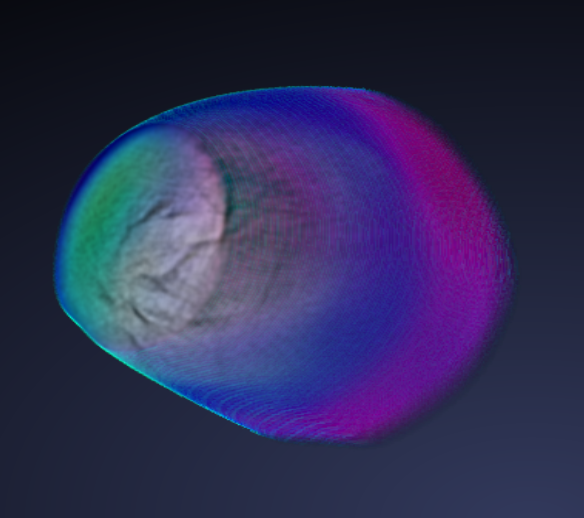
\includegraphics[scale=0.4]{img/usct1}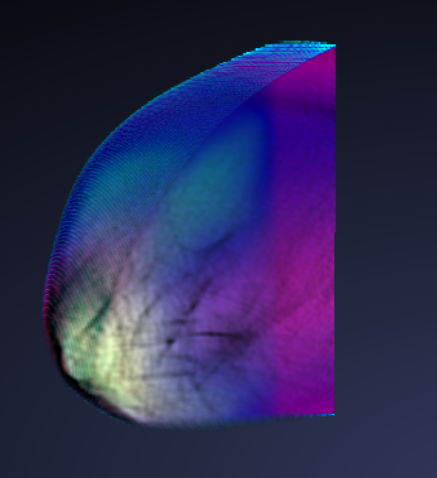
\includegraphics[scale=0.4335]{img/usct2}\\
\caption{Volume visualisation of breast phantom made by USCT}
\end{figure}
%USCT VIS

The very first steps in modern computer graphics was made by me during the project. The first experience in work with WebGL was gained during customisation of the Tomo Ray Caster. GLSL as my first shader language was learned during the work. A lot of knowledge about image processing and scientific data visualisation, which became the basis for my thesis work was received by me at the workplacement.

%INTERNSHIP REPORT

\section{Arction Oy and Ligthning Chart}

Arction Oy is a Finnish software company based in Kuopio. Their team has a strong background in computer graphics and science. The main product of the company called LightningChart Ultimate. It is the fastest C\# library for scientific and engineering data visualisation. The library is capable to draw massive XY, Polar, Smith and 3D XYZ graphs, polygonal mesh models, surfaces, 3D pies/donuts and Geographic information. The library has an API for .NET WinForm and WPF applications, it is also possible to use it for a traditional Win32 C++ software development. The main advantage of the library is the fact that it is based on low-level DirectX graphics routines developed by Arction, then the most part of competitors use graphics routines which belongs to System.Windows.Media.\\
\begin{figure}[!h]
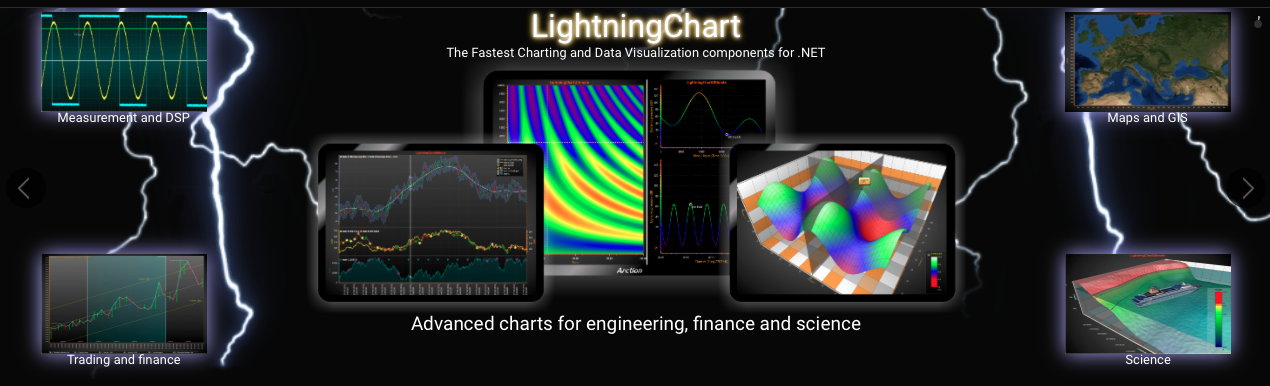
\includegraphics[scale=0.33]{img/lchu}\\
\caption{Example of LightningChart possibilities from the main page of Acrtion}
\end{figure}
%arction website

\section{Project Goals}

So, as it can be concluded from the previous section, LightningChart is a very advanced software for 3D rendering based on polygons and lines. That's why, an idea to extend it by the special rendering engine for visualisation of volumetric data was suggested by me to the CEO of the company. It will give Arction's clients the unique possibility to combine visualisation of volume datasets with a wide range of other 3D possibilities provided by the library. \\

The rendering engine must be able:
\begin{itemize} 
\item to render large multi-dimensional volumes with an interactive frame rate.
\item to move and rotate the model in the chart's space.
\item to provide clients with possibilities to apply windowing and thresholding to the initial dataset.
\item to render the model semi-transparent.
\end{itemize}

Basically, this tool will give end users possibilities to change the contrast and brightness of the model's visualisation for better recognition of tiny details and make areas, which are out off certain range, totally transparent. It will also reveal insights into the internal structure of the model to the user via semi-transparency.

\chapter{THEORY}

This chapter explains the theory behind the project. It should introduce the main concepts of computer graphics, specify the difference between polygonal mesh model and volume rendering. It also contains an overview of different volume rendering techniques with their advantages and disadvantages in terms of speed, final image quality, flexibility and other implementation issues.

\section{Rendering}

Visualisation of 3D object as 2D image called rendering. Usually, 2D image is based on pixels\footnote{a shortcut from picture element}. In case of a grayscale picture, it is a two-dimensional array and the value of the array elements represents the brightness of corresponding pixels on a screen. Configuration of colored images is dependent from a color model, the most popular one is RGB. It represents an image as three different grayscale pictures for three different colors called channels. In case of the RGB color model the images contain Red, Green and Blue values, sometimes it also keeps an informant about opacity and the channel called Alpha.\\

Color model is the mathematical abstraction which allows computers to calculate brightness of a corresponding point on the screen. RGB is the original one for modern computer graphics, because it represents colors in the way they are physically reproduced on screen. There are several other color models. They have their own advantages, for example, some of them gives us an advanced editing possibilities while others represent physical characteristic of different types of output devices like printers.\\

Multidimensional data can be represented in two different ways: as a surface and as volume. Future in this chapter, we are going to talk about these two concepts a little bit closer. We will highlight their advantage and disadvantages, common and uncommon features. Moreover, we are going to discuss an implementation detail of the techniques on modern hardware.

%https://www.artstation.com/artist/vidarrapp illustration


\section{Polygonal Rendering}

Today we are literally surrounded by the surface rendering based on polygonal mesh. The technology is used in computer games, design, cinema, science, engineering and etc. The technology is so popular that entire 3D graphic pipeline is built around the idea. That's why this type of visualization is easily accelerated by graphic cards.\\

\subsection{Vertexs}
Traditionally, 3D surfaces are constructed out of huge amount of polygons connected as a mesh. Due to simplicity, they usually have a triangular shape. It is possible to describe triangle via list of three coordinates called vertices. The internal area of the shape filled with color during rasterization step. The color is calculated as dot product between the surface vector normal and the vector of light.
%http://people.csail.mit.edu/fredo/Depiction/1_Introduction/reviewGraphics.pdf

\begin{figure}[!h]
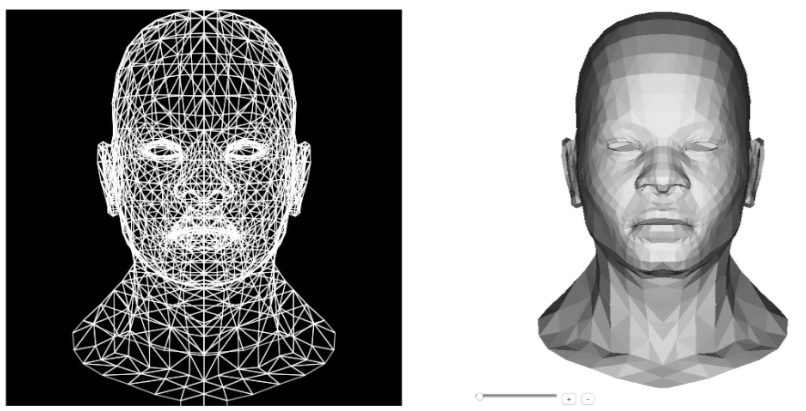
\includegraphics[scale=0.55]{img/mesh}\\
\caption{Wireframe and flat shading polygonal meshmodel}
\end{figure}

\subsection{Normals}
Surface normal vector of a triangle can be calculated as a cross product of two triangle's sides, but it will give an acceptable result only for very flat surfaces. That's why curve surfaces usually contain an additional normal vector for every vertex. They are able to significantly improve detailisation on the model. The information kept in them is used during shading and the tessellation of the model's geometry.\\

%http://www.emeyex.com/site/tuts/VertexNormals.pdf

\subsection{Textures}
Very small details can be added to the model via textures. It is specific 2D image which is used to sample high frequency information during rendering. The picture usually contains local color values, but it also can carry an information about normal vectors for a nice visualisation of very small structures on the surface. Textures are mapped to the surface via third vertex' parameter called texture coordinates. They keep an information about corresponding to this vector position in the 2D space of the image.\\

%http://www.dcs.ed.ac.uk/teaching/cs4/www/graphics/Web/advanced_ogl.pdf

\subsection{Redering process}
Position, scale, rotation of the object and perspective characteristics of the space is specified via matrixes $4\times4$.\\

%http://www.tutorialspoint.com/computer_graphics/3d_transformation.htm

Specific program called shader receives all the information together with a camera and light source positions, after that they are able to perform calculations needed to render the final image in accord with the goals of the visualisation. Usually, the calculations are produced by graphic card in a parallel way.

\section{Volume Rendering}

Volume data are composed out of voxels\footnote{volume element}. Voxel is simply a point in 3D space, which has a position and a color. Together gives us an opportunity to visualise up to six scalar parameters. There are two ways to render volumes. We are going to discuss about main principles, advantages and disadvantages of the technologies in this section.\\
%shear-warp paper 3

\subsection{Indirect}

The first one called indirect volume rendering. It is based on the idea that it is possible to extract surface out of the dataset during preprocessing and render the surface as a polygonal mesh. Several algorithms are invented for this application:
\begin{itemize}
\item Marching Cubes
\item Surface Tracking
\item Fourier Transfor Rendering
\end{itemize}
It is the oldest idea behind volume rendering and it has plenty of disadvantages:
\begin{itemize}
\item complex and slow preprocessing algorithms
\item can be inacurate due to noise
\item sometimes does not able to generate isosurface out of specific dataset, for example smoke
\item lose an information about an internal structure
\item need to repeat preprocessing to apply changes in a transfer function
\end{itemize}

But the algorithm is very popular for generation of medical illustrations, video or other static visualisation. The main advantage of the solution is that nicely preprocessed model can be easily rendered in via wel-known 3D mesh models' rendering, even in very weak hardware.\\

Unfortunately, this technology is not suitable for our project, because it does not satisfy our requirements.
%http://www.forceflow.be/wp-content/uploads/2012/02/vr_overview.pdf

\subsection{Direct}
Direct volume rendering does not require any preprocessing. The data is visualised from an original dataset. It gives the algorithms an opportunity to modify a transfer function runtime. There are four most common technics for direct volume rendering algortithms, which will be discussed more detailed future at the section.\\

For an implementation of hardware acceleration for redering process a volume data has to be loaded to the grapic cards. It is usually served as 3D texture or as set of 2D textures. Several slices can be collected to one huge texture map due to optimization of  a texture's buffer consumption. 

%http://www.forceflow.be/wp-content/uploads/2012/02/vr_overview.pdf
\subsubsection{Texture-based}

As it was mentioned befor the graphics pipeline of modern graphic cards is optimized for rendering of polygonal mesh models. So, volume rendering algorithms are forced to use the set of tools to achieve hardware acceleration. Texture-based volume rendering is the most straight forward way to achive the aim.\\

As it was already said textures are used to add tiny details to polygonal models. Any graphic library has an advanced set of tools for texture mapping, which can be used to this kind of volume rendering. The algorithm creates set of planes called proxy geometry. Transfer function projects the volumetric dataset on the proxy geometry. The final image is rendered out of the planes with applied on them textures via Alpha-blending.\\

%http://http.developer.nvidia.com/GPUGems/gpugems_ch39.html
A proxy geometry can be created in two different ways. The first one called 2D texture-based rendering. In this case three different sets of planes are generated. All sets are generated perpendicular to a different directions in 3D space. This approach leads us to sudden jumps in image quality for different camera position and does not allow to change the sampling rate of the visualisation.\\
\begin{figure}[!h]
\centerline{
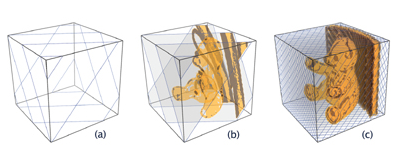
\includegraphics[scale=0.7]{img/texture-based}
}
\caption{a) example of proxy geometry for 3D texture-based volume rendering a) Texture-based volume rendering with a lower sampling rate c) high sampling rate texture-based volume rendering}
\end{figure}
That's why the second way was invented. It is called 3D texture-based volume rendering. In this solution the algorithm creates only one set of planes which are always perpendicular to the camera and textures are mapped on them differently for different camera position. \\

It gets rid of an artifact of the first technique and allows to modify the sampling rate of the visualisation. The approach is the most popular direct volume rendering algorithm among medical software, but it was not selected for Arction's Volume rendering engine, because it is less flexible than all other methods discussed further. It is possible to use transfer function to emphasize or classify features of interest in the volume, but it is not comparable with possibilities provided by other approaches.
%http://www.forceflow.be/wp-content/uploads/2012/02/vr_overview.pdf

\subsubsection{Ray Casting}

Image is produced by the algorithm throughout sampling of the volume along tracks of the rays which travel inside the dataset. A smiple realisation of hardware acceleration of the aproach requer generation of boundaries for our volume. Usually they are represented by cube. \\

Volume Ray Casting includes four simple steps:
\begin{itemize}
\item An engine shoots a ray in a direction of observation for every point on a screen.
\item The ray travels throught scene and dataset.
\item A vector of the ray's track is calculated based on position there the ray hits front and back faces of the cube.
\item The volume is downsampled along the ray track and color of the pixel is calculated out of collected information in according with a Ray Function.
\end{itemize}
\begin{figure}[!h]
\centerline{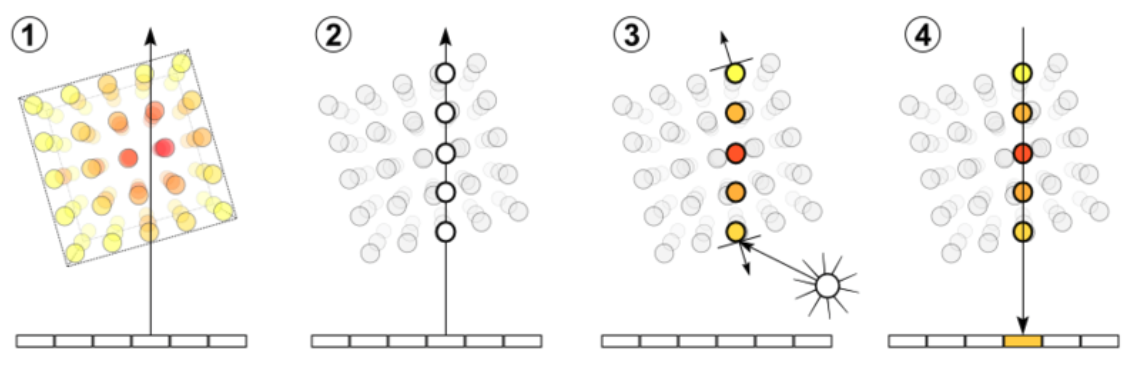
\includegraphics[scale=0.35]{img/rayCast}}
\caption{Raycasting steps: 1) The ray is shooted, 2) The ray travels throught scene and dataset. 3) Inlet and outlet position of the ray's track are detected 4) Downsampling and the pixel's color calculation process}
\end{figure}

Ray Function is a core of the algorithm. It possesses an entier power of the technique, because it specifes the way how the data is combined. Such a high level of flexibility is provided to the algorigth by Ray Function. It is very powerful tool for feature extraction, becuase it controls how color, opacity and gradient of isosurface are calculated by the enigene. Transfer function and classification are also performed via Ray Function.\\

The algorithm has very high rendering quality without any additional arifacts. Due to the reasone that every ray is calculated seperatly it is easilly implemented in modern hardware focused on parallel calculations. The main problem of the algorith is that rays usually do not hit the voxel to the center. In case of 3D space an interpolation is a very complex operation in terms of calculanal expensis, which has to be performed to get nice sampling.
\subsubsection{Splatting}

The technique was created to reduce interpolation expensis which were the main problem of Volume Ray Casting. The solution uses totally oposite aproach to reach the goal. Instead of sampling of the dataset by ray, the algorigthm projects the voxel to the image plane one by one. Of course the voxel porjections do not always fit excatly to pixels' grid of screen, but the problem is again solved by an interpolation, fortunately in this case the operation is much less expensive in term of calculation, becaus it is perfomed in 2D space. \\

The final pixel's color is calculated in a very similar way used by Ray Function, that is why the algorithm is as flexible as Volume Ray Casting. The main disadvanrage of the approach is that some artifacts are contributesd to the final image due to voxels overlap. It is also difficalt to change sampling rate of the approach. The issues make the algorithm less interesting for us.

\subsubsection{Shear-warp}

As Splatting, the aproach also tries to speed Ray Caster up by solving of the interpolation issue, but it uses totally different way to illuminate the problem. Shear-warp has a very similar idea to the Volume Ray Casting. In some sence it is an optomozation of the technique which makes rays always hit excatly to the center of voxel.\\

The aim is achived by transformation of the volume data to sheared object space by translation and scaling of slices. After that an intermediat 2D image is produced by Ray Casting performed in the sheared object space. The transformation brings some distortion to the output image. It is fixed at last step of the algorithm called wraping. Final image is result of transformation applied to the intermideia picture.\\
\begin{figure}[!h]
\centerline{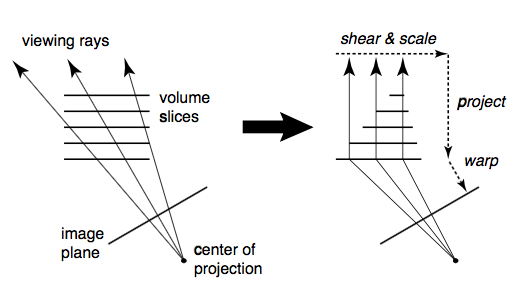
\includegraphics[scale=0.5]{img/shear-warp}}
\caption{(left)Ray Casting in world coorinates, (right)Ray Casting in shear object coordinates}
\end{figure}
This solution gives us the fastest volume rendering process, but unfortunatly the algorthm also suffers from several types of artifacts. Some of them are result of sampling rate inconsistent along different directions, others are produced by 2D transformation at wrapping stage.

\chapter{IMPLEMENTATION}
This chapter contains detailed explanation of the product implementation. It discribes how the engine works, what kind of parts contains and which tools are used in it. Key step of the engine work are highlighted and explaned in this chapter.\\

In according with results of literature research several the most commone algorithms for volume redering were comparied and the most siutable approch was implemented as Volume Rendering Add-On of LigthinghChart Ultimate. One of the main requerment for the LightningChart's volume rendering engine is possiblity to combine volume and other 3D visualisation at the same chart space. Easy and accurate convertion between volume and chart coordinate system is needed. The volume ray caster and texture-based volume rendering can provide us with the feature. The algorighms keep entier visualisation inside the coordinate system of a proxy geometry. It is placed on the coordinate system of chart. It means that the coordinates of volume model can be easilly converted to the coordinates of enier chart.\\

Anouther important thing is implementation of rotation, scaling and transmition of the model in the chart space. As it was already mentioned the proxy geometry also makes it much easier. But this approach is not fully applieable for 3D Texture-based solution. In this approach slices always have to be perpendicular to the camera, that is why rotation has to be implemented on the process of texture mapping.\\

Finally there are only two technologies. The final chose is Ray Casting, because it has better image quality than 2D Texture-based rendering. In addtition, Texture-based volume rendering is less flexible than Volume Ray Casting.
\section{Tools}
This part of the chapter discibes technologies used in the implementation of the project. It also gives a short explation to thier usage in the solution. The rendering engine has to became a part of LightningChart Ultimate. An integration with the library gives some restrictions in terms of set of tools which can be used in the project and it plays a key role in technology selection.
\subsection{C\# and .NET}
C\# is general perpuse  multi-paradigm programing language with strong types. It is created by Microsoft as native language of .NET Framework. Our days the language can be used for Web services, Windows desk-top and mobile applications, computer games with several different game engines. In addition, Xamarin created set of tools for croos-platfom C\# development.\\
%xamarin.com

In some sence it contains constructions ispiered by an object-oriented, imperative, functional and many other programming paradigm. The language belongs to C-like family, that is why the curly-brace syntax looks very similar to the C, C++, Java.  C\# combines an advantages of Java and C++ in single powerful and elegant way. It is more simple and safe than C++, but at the same times it has advanced features like: pointers arithmetics, enumerations, lambda expressions, structs, delegates and implicitly typed local variables. Even today when the most part of them are implemented in the last version of Java, C\# still is way more flexible.\\

Other advanced feature of C\# is Language-Integrated Query expressions or shortly LINQ, it is set of functions for strong-typed queries, which allows to write very short functional stylied code for collection processing.\\

.NET Framwork contains applications run in virtual execution system called the Common Language Runtime shortly CLR and more than 4000 of class which implements wide range of useful functionalities. The runtime is able to execute an Intermediate Language, which is compiled from C\# or 20 other languages.
%https://msdn.microsoft.com/en-us/library/z1zx9t92.aspx

C\# is used in the porject for as close as it is possible intergration with LightningChart Ultimate. It performes loadign and preprocessing of the dataset and management of visualisation process.

\subsection{DirectX 11}

DirectX is a C/C++ API\footnote{Application Programming Interface} for work with multimedia resources created by Microsoft for Windows and Xbox. It contains advanced tools for rednering of 2D and 3D graphic and sound management. Direct3D is a part of the library responsible for hardware accelerated rendering of 3D graphics. The tool is mainly focused on GPU accelerated rendering of polygonal meshmodels.\\
%http://searchwindowsserver.techtarget.com/definition/DirectX
 \begin{figure}[!h]
\centerline{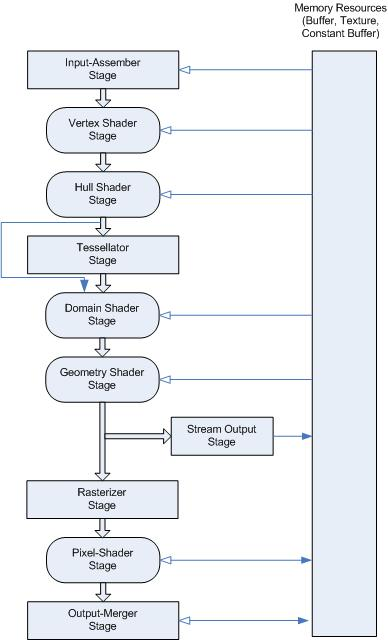
\includegraphics[scale=0.9]{img/pipeline}}
\caption{Flowchart of Direct3D 11 Graphics Pipeline\label{fig:pipeline}}
\end{figure}
\subsubsection{Rendering Pipeline}
Key consept of the library is redering pipeline. It is a very general term in computer grapics. The pipeline is a siqence of stages which recieves an input data as set of polygons, textures and variables, process the information step by step and generates the final image in the end.\\

Direct3D's pipeline has two types of steps:
\begin{itemize}
\item Fixed-function - perform certain processing operation which can be customize due to some level thougth the API.
\item Programmable - processing is performed by so called shader program. It is function which is created by developer and satisfies input and output parameters of the stage.
\end{itemize}

The graphics pipeline is shown on Figure \ref{fig:pipeline}. Boxes with rounded angles represent programable stages and other ones are fixed-functions. Let me exaplain every step of the pipeline more detailed: 

\begin{itemize}
\item Input-Assembler Stage recieve input information as set of buffers and supply future to the pipeline. There are four types of buffers in Direct3D:
  \begin{itemize}
    \item Vertex Buffer is used to define geometry of the object by list of vertexs. Every vertex has to follow Input Layout deffined for the pipeline by developer. It discribes the vertex members like: position and texture coordinates, color value, normal etc used in this application.
    \item Index Buffer conatins an order of vertexs as sequence of integer variables.
    \item Constant supplies pipeline with a constant data, like transfor matrixes, position and directions of ligth sources, textures, and so on.
    %https://msdn.microsoft.com/en-us/library/windows/desktop/ff476898(v=vs.85).aspx
  \end{itemize}
\item Vertex-Shader Stage is the first programmable stage of the pipeline. Verteces are read one by one and processed in according with Vertex Shader program supplied by developer. For best performence the processing has to includes every operation which can be performed on every vertex indivudualy. The function is not able to destroy or create new vertex.

%книга
\item Hull Shader, Tessellator and Domain Shader stage are used togher to archive tessellation\footnote{Process of mesh model's enchantment via aoutomatic generation of additional polygons} of the mesh.
  \begin{itemize}
    \item Hull Shader programm includes two functions. The first one recieve primitives and calculates tessellation factors out of the data. The second function is called once for every contorl point and creates them.
    %книга
    \item Tessellator uses data provided by Hull Shader and one of several algorithms to choose the best point to break of current primitive into smaller polygons.
    \item Domain Shader uses an original infromation from Hull Shader toughert with results of tessellator to generate new verteces list.
  \end{itemize}
\item Geometry Shader recieves several verteces at the same times and perform operations on them. An ability to add and remove points from pipeline makes the function extimly powerful and flexible tool. For example it can easelly turn single vertex to the polygon of even set of polygons. It is able to pass geomtry future along pipeline or away to output stream.
\item Rasterization projects geometry to the final image and determines which pixels are covered by the polygons. It interpolates the verteces' atributes inside the primitives to get the pixels values for the area. It also perfoms depth and stencil tests.
\item Pixel shader is executed once for every pixel on the output target. It is supplied with an information from Resterizetion step and calculates per pixel data for example color of imga's points. Usually texture sampling and hight quality lightning calculations are implemented by pixel shaders.
\item Output-Merge Stage uses pixel shader's output togher with depth/stencil information to generate final image and write it in appropriate way to render target.
\end{itemize}

It is worth to metntion that a render terget is not always represented by screen. Sometimes the output is stored in texture. For example the image can be loaded again to graphic card and sampled to get some precalculated prevously information. The technique called miltyi-pass rendering.

%https://msdn.microsoft.com/en-us/library/windows/desktop/ff476882(v=vs.85).aspx
\subsubsection{HLSL}
There are two way of rendering pipeline customization. Fixed-functions behavoure can be modified by the API and programable stages flexiblities is orgonised via special type of programming languages called Shader Languages. Direct3D's realisation of shader language called HLSL\footnote{High Level Shader Language}.\\

The language is basically significantly modified version of C. The lanaguage does not support features like pointer artichmetics and dynamic momory allocation, but the syntax is still understandable for C developers. It extends C syntax by classes, several new data types, buffers, sematics and huge library of useful for shader development functions. There are vector, matrix and 1D-3D texture data types which are very useful for processing of 3D primitives. As it was already mentioned buffers are used to supply pipeline with data. Sematics contains metadata which is related with data exchange among fixed-function and programable stages of the pipeline.
\subsection{SharpDX}

As it was already mentioned DirectX is C++ library, so it is not possible to use in directly from C\#. The problem is solved by SharpDX. It is open-source managed C\# wrapper for an original API of DirectX. It plays role of bridge between API and .NET. As result developers are able to manipulate the functionality of the API  from C\#.\\
%http://sharpdx.org
Every feature of the API is implemented in a very natural way. That is why a huge amount of tutorials and example avable for original C++ API can be easylly translatted to C\# and SharpDX. Even original documentaion is still useable for SharpDX development.

\subsection{LightningChart Ultimate}

LightningChart Ultimate is the fastest C\# library for scientific and engineering data visualisation. It is able to draw massive XY, Polar, Smith and 3D XYZ graphs, polygonal mesh models, surfaces, 3D pies/donuts and Geographic information. 

\begin{figure}[!h]
\centerline{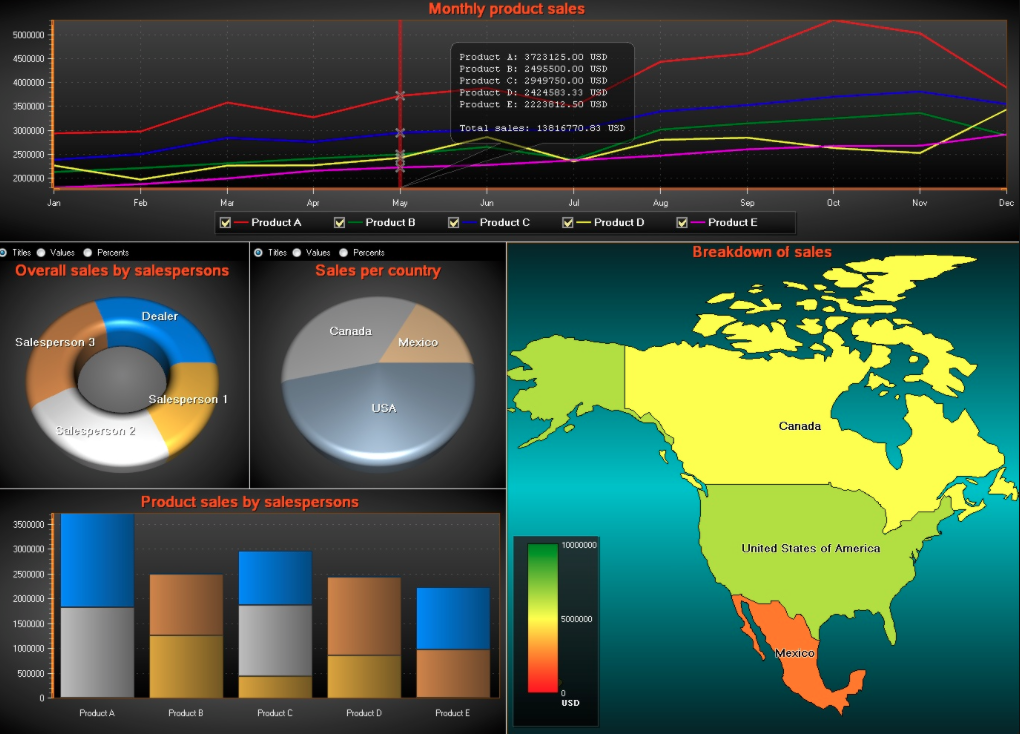
\includegraphics[scale=0.4]{img/chart}}
\caption{Some of LightningChart Examples}
\end{figure}

The library has an API for .NET WinForm and WPF applications, it is also possible to use it for a traditional Win32 C++ software development. The main advantage of the library is the fact that it is based on low-level DirectX graphics routines developed by Arction, then the most part of competitors use graphics routines which belongs to System.Windows.Media.\\

An intergration with LightningChart has sevral advantages and disadvantages. In one hand, it applies main role in terms of tools selection for project implementation, because deep enough integration can be achived only via usage of exactly same set of techologies. It also  forces the volume rendering engine to follow similar class arcitecture. Moreover, LightningChart is commercial software package. That is why any external dependences have to be avoided as much as it is possible. It means that even open-source libraries can not be used without extrimly important reason.\\
%http://arction.com/products_lc_ultimate_sdk

On the another hand an abilities of LightningChart to draw 3D polygonal mesh models make the development much more simple. The library is able to rotate, scale and move the models around chart's space, so the functionality can be easilly applied to proxy geometry. As result the features are implemented without almost any development from the side of volume rendering engine. In addition it is a huge advantage for clients, because volume and mesh 3D models can be visulised at the same chart in the same coordinate system. It provides them with really uniqe and powerful opportinity for complex 3D visualisations.

\section{Visualisation process}

This section of the paper explaines main principles and implementation detailes of the project. It disribes the main challangs and explain how were solved during development of the rendering engine.

\subsection{Loading and preprocessing of dataset}
The most commune way of volume data distribution is collection of 2D slices. The 2D slices are just images in common format. Sometimes they can be represented as set of DICOM\footnote{Digital Imaging and Communications in Medicine} files. In this case they contain metadata of the studies toughere with embeded picture. Volumes can also be distibuted as table of original values. The table usually is part of RAW file which also contain some meta information. Actually, RAW is several different format with commone name and more detialed specification of every single approach depends from machine which perfomed the data aqusition.\\
\begin{figure}[!h]
\centerline{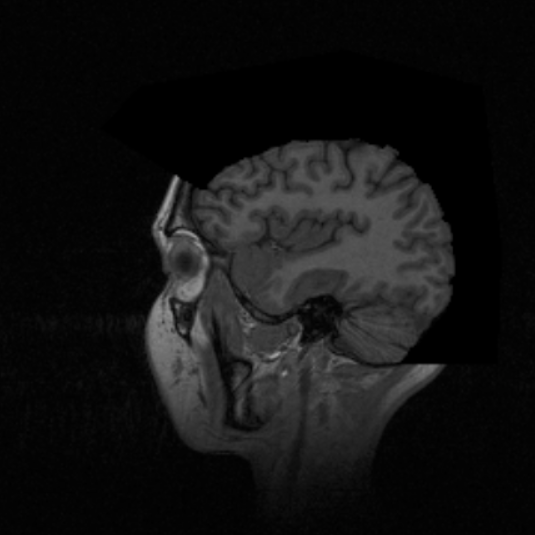
\includegraphics[scale = 0.35]{img/slice}}
\caption{Single slice from Volume dataset.\label{fig:slice}}
\end{figure}
Unfortunatly, current implementation of the volume rendering engine supports only first approach, because slice-based data is easier to get. Specific software can converte DICOM slices to the picture formats supported by .NET like *.JPEG, *.TIFF and *.PNG. RAW volume data files can be converted to *.CSV files, but due to the reason that there are many different specifications of the files it is very difficalt fo find the software.\\

.NET tools for file handling load images in supported by framework formats. The slices are loaded to the memory from specified folder as an array of bitmaps in the same order they are already stored. An example of slice is shown on Fugire \label{fig:slice}. DirectX 11 also supports 3D textures, but the approch was not used in the engine, becuase the feature is not supported by DirectX 9. Arction wanted to have an opportunity to port the volume engine to DirectX 9 quickly, if it would be needed. \\

\begin{figure}[!h]
\centerline{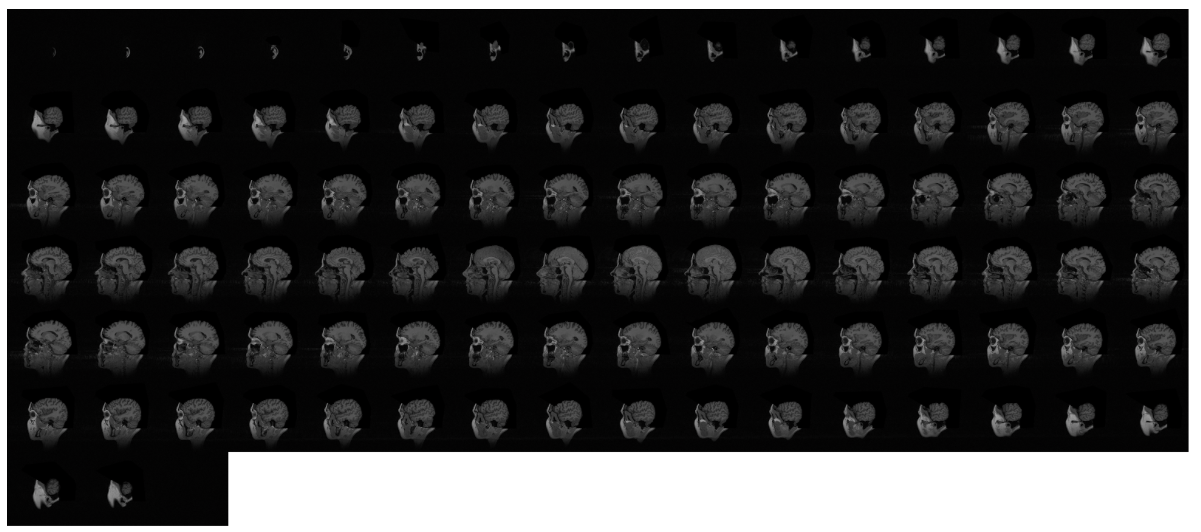
\includegraphics[scale = 0.35]{img/map}}
\caption{An example of slice map\label{fig:map}}
\end{figure}
Texture buffers have a limmited amount of avaible slot. Slices usually have a very low resolution so it is not efficent to load them one by one, due to an optimization of texture buffers' consumption an array of slices is mapped to the big texture map. The map contains slices mapped from left to right in according with an array index, look Figure \label{fig:map}. A bitmap processing is accelerated via pointer arifmetic, but any way it requers some time. That is why the engine is also able to load preprocessed texture map for quicker start of visualisation. \\

\begin{table*}[!h]
 \begin{center}
    \begin{tabular}{ c  c }
    \multicolumn{2}{l}{TABLE 3.1: Characterisation of different technologies \label{tab:level}}\\
    Feature level & Maximal size of texture map\\
    \hline
    9\_2 & 2048\\
    9\_3 & 4096\\
    10\_0 & 8192\\
    10\_1 & 8192\\
    11\_0 & 16384\\
    11\_1 & 16384\\
    12\_0 & 16384\\
    \end{tabular}

  \end{center}
\end{table*}
DirectX has a limmitation in terms of the biggest avaible texture size, which can be loaded to the graphic card. The value depends from feature level of the graphic card, look table 3.1. Featue level defines the functionality supported by the graphic card. Usually, modern graphic cards have at least 11\_0. It means that they supprot up to 16 384 pixels per side. Sich a big texture can keep volume dataset with more than 600 voxel long in every dimenssion. It is possible to render even bigger models, because several texture maps can be generated if it is not possible to fit entier data into single one.\\
%https://msdn.microsoft.com/en-us/library/windows/desktop/ff476876(v=vs.85).aspx

\subsection{Multi-pass rendering}

Possibility to render scene in several steps makes rendering pipeline especially flexible. The technique called Multi-pass rendering. Sometimes it is more efficient to render scene in several steps. Multi-pass rendering is based on an idea that every step excpet the last one outputs the result of perfomed calculation to to texture. The final pass sample information from the set of textures and generates the final image.\\

Deferred rendering is one of the most popular realisatiom of the idea. The technology is created for rednering of scenes with large amount of dynamic lights. Traditionaly this kind of functionality requers a cemplex set of shaders. Multi-pass approach breaks the process to smaller peaces and perfomes the calculations separatly for every step. It allows to simplify an architcture of rendering framework. It can also give an opportunity to apply GPI acceleration to some parts of rendering algorithm which used to be executed on CPU befor.\\

Our volume ray caster is also going to get some advantages from multi-pass rendering. In case of the solution it has only two passes and it allows the algorith to determine vectors of the sampling ray in the volume coordinate system without any additional mathematical calculations. It means that entier rendering pipeline of the engine contains two typical rednering pipelines. The first one is generates tecxture which contains an important information for rendering of final image at the second pass. Both passes use only vertex and pixel shader programs.

\subsection{First pass}

At this step rendering engine has to generate texture which keeps an information about the exit position of sampling rays. For this reason front-face culling mode of Direct3D has to be turned on. It makes the library to draw only polygons which are normally not visualised, because their front side looks in an opposite to the screen's direction.\\

An input of the first pass contains only set of vertecs for boundries of the dataset, constant buffers for slice range clipping and matrixs for calculatuin of the vertecs position of the chart space. The boundaries are always renpresened by cube. The cube contains 8 verteces calculated on C\# according with requered size of the volume model. Constant buffer is represented by two Vector3 variables, one of them contains the number of minimal slice for every direction and another one keeps an information about maximal boundaries. We also have three traditional for 3D graphic Matrixes: World Coordinate, View, and Projection. This matrixes have uque values for every object and allows to calculate desierable position, scale and rotation of the object in  screen coordinats.\\

The Vertex Shader of the first pass calculates positions of the cube verteces in accodring with clipping range buffers. After that matrixes are applied to transform the geometry to the screen coordinates. Internal coordinates of the dataset are calctulated out an original position of verteces. They are represented by Vector3, with value range from 0 to 1 along every axis and stored as texture coordonates.\\

The Pixel Shader represents the coordinates as color. X coordinate is stored in red chanel, Y one is stored in green channel and Z coordinates is stored as blue value. The final result of the first pass is demostrated on Figure \ref{fig:first}.
\begin{figure}[!h]
\centerline{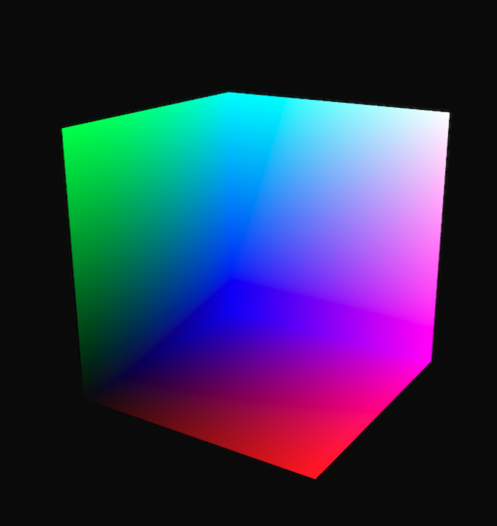
\includegraphics[scale = 0.5]{img/first}}
\caption{First pass output\label{fig:first}}
\end{figure}

\subsection{Second pass}

At this pass the engine has to calculate vector of sampling ray displaisment thougnt dataset. The enter coordinates of the rays are need for the calculation that is why defult culling mode has to be restored. The input of the pipeline has a set of vertecs, matrixs, an original dataset represeted as texture map, texture rendered at the first pass, buffers with slice range, contrast, brighness and tresholds setting.\\
\begin{figure}[!h]
\centerline{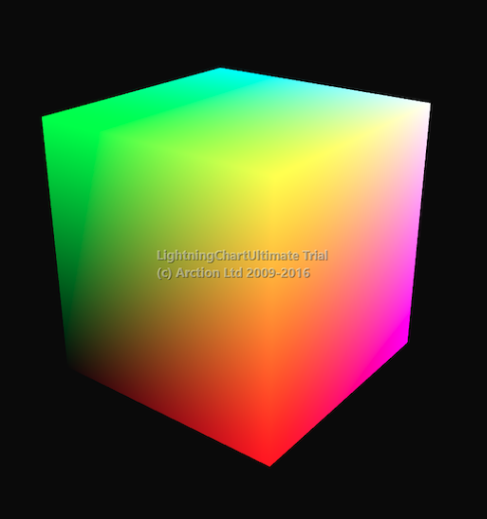
\includegraphics[scale = 0.5]{img/second}}
\caption{Coordinates of the hit points.\label{fig:second}}
\end{figure}

Second pass has excatly same vertex shader with the first one, but due to changes in culling mode it output enter point of sampling rays. In other word the coordinates of the points there the rays hit the boundaries. Firgue \ref{fig:second} shows them at the same way it was done on the first pass.\\

The pixel shader samples coordinates there rays hit the back side of cube from the texture generated at the first pass. After that it substracts enter coordinates calculated at the vertex shader of the second pass from the information. The operation result is the vector of the rays track. The tracks are visulised as colors on the figure \ref{fig:final} The vector is devided by sampling rate to get step vector. 
\begin{figure}[!h]
\centerline{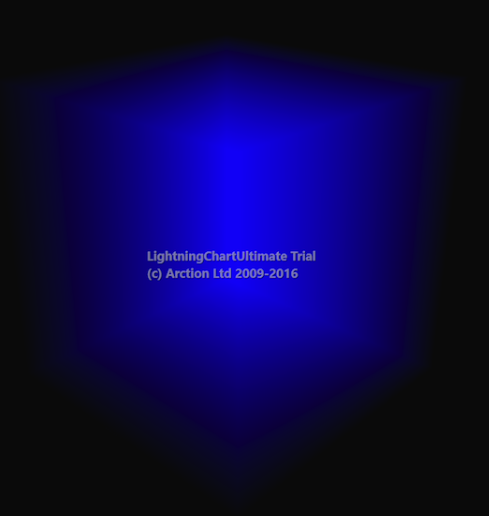
\includegraphics[scale = 0.5]{img/final}}
\caption{The visualisation of sampling ray vectors' tracks \label{fig:final}}
\end{figure}
Acruall volume sampling is prefomed by for loop. It starts from the hit point of the ray and adds a step vector every interation to get coordinates of new sampling point. The data is sampled out of volume by function which calculates correspondent position on the texture map.\\

It calculates the nearest slice coorespondent to the Z position. After that it checks how many full rows are included in to the value and what is the column number of the rest. Values from two closest slices can be interpolated to get smoother result. Handling of the information depends from Ray Function.\\

\subsubsection{Empty space skipping}

The most part of volume dataset is represented by an empty space. Empty space does not contain any importan information, usually it is represented by pixel with a very low value per each chenalle. In our case a voxel is classified as empty one if its values is out of a treshold range for all of its channels. There are huge amount of rays which travels thought arrays which contains only empty space. The optimization has to prevent high resolution downsampling of the regions.\\

Due to realisation of the technique, the sampling is brouken down into two steps. At the first step ray travels thougnt dataset with a very low sampling rate. It saves positions of the first and the last non-empty voxel hitted by the ray. After another ray goes thougt the dataset with a higher sampling rate. The second ray starts one low resolution sampling rate step vector earlier than the position of the first non-empty voxel. It stops one low resolution sampling rate step vector after the last non-emtpry voxel detected by the first ray. The process is shown on figire \ref{fig:empty}.\\

\begin{figure}[!h]
\centerline{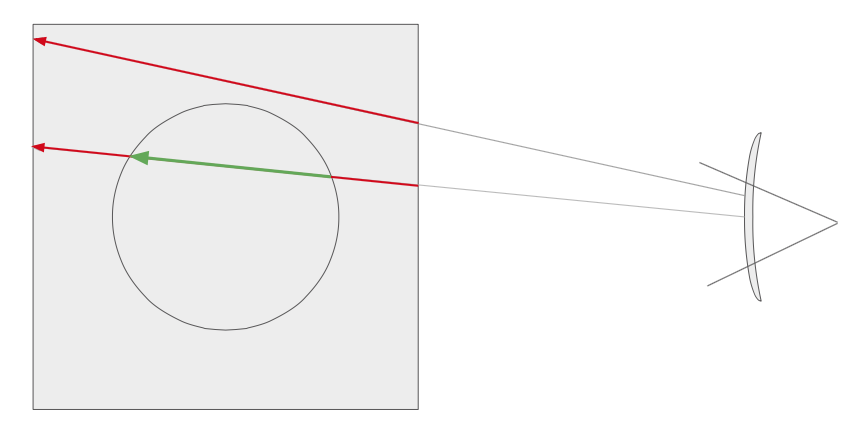
\includegraphics[scale = 0.5]{img/empty}}
\caption{Red arrows represents low resolution sampling rate ray. Green demostrates high resolution sampling one.\label{fig:empty}}
\end{figure}

High and low resolution sampling rates are spcified by constant buffers. High sampling rate determines rendering quality. An optimal quallity is reached then it mutch an amount of voxels in the longest dimmension, because it allows to performe uniform sampling of entier dataset and collect all information stored inside. Low resolution sampling can only be defined via experiment. Too small low resolution sampling rate can contibute some artifact to the final visualistion. It is a trade of quality and frame rate. The rigth value have to keep an intertive framerate and unnoticable artifacts.


\subsubsection{Ray function}

Ray function determines how the sampled data is combined. Different ray functions allows to extract diffrent features out of the dataset. Two most commune ray function are implemented in out rendering engine.

Accomulation function uses alpha-compositing to get compose as much data as it is possibel. The visualisations produced by the technique look like semi-transperent gel. Ray function implementation is represented by for loop, which runs from 0 to the value sampling rate. Every interation contains several steps:
\begin{itemize}
\item The voxel is sampled out of texture map.
\item The volel's value validation is performed by if-statement. It checks that every chennal is in its personal treashold range. If the voxel is empty next four steps have to be skipped.
\item The alpha is calculated in according with an equation:
\begin{equation} \label{eq:alpha}
\alpha_{output} = \alpha \times opacity \times \frac {1}{{sampling\ rate}}
\end{equation}

\item The colors are calculated in according with an equation:
\begin{equation} \label{eq:color}
color_{output} = (1 - \alpha_{accomulation}) \times (color + brighness) \times contrast  \times \alpha
\end{equation}\\

$\alpha_{accomulation}$ contains previosuly accomulated alpha values. Brighness and contrast are supplied by constant buffers and used to perform windowing.
\item After that the colors and alpha are added to the correcpondent variable which keeps a previousl accomulated infromation.
\item If-statement checks that alpha is not oversaturated. The ray has to be terminated in this case.
\item Step vector is added to reach next sampling position.
\end{itemize}

An example of images produced by an accomulation function is demostrated on figure \ref{fig:accum}.\\

\begin{figure}[!h]
\centerline{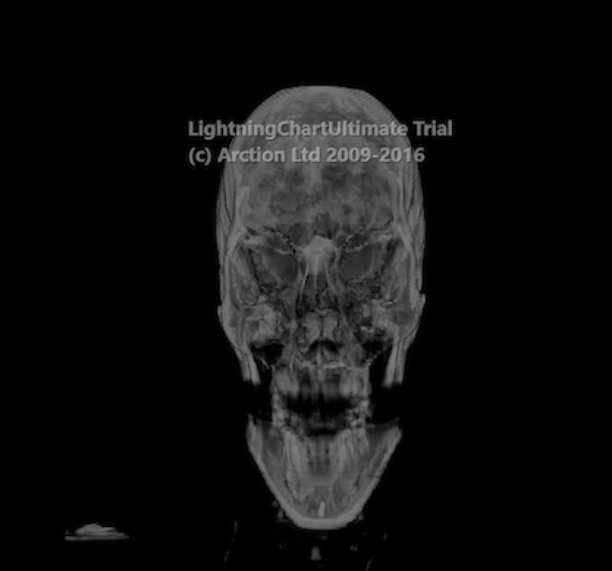
\includegraphics[scale = 0.6]{img/accum}}
\caption{An example of an accomulation function output\label{fig:accum}}
\end{figure}

Maximal intesnsity visualise only the brightest value sampled by ray. It gives very similar result to the X-ray images. The ray function is very similar to the prevouse one. It also use for loop and step vector to sample the dataset, but it does not accomulate the information as it is done in previous example. Instead it keeps the biggest value which ray meet during the travel and put it to the pixel in the end. It allows end user to idetify specific structures inside the volume. An example of the ray function result is shown in the figure \ref{fig:maxi}

\begin{figure}[!h]
\centerline{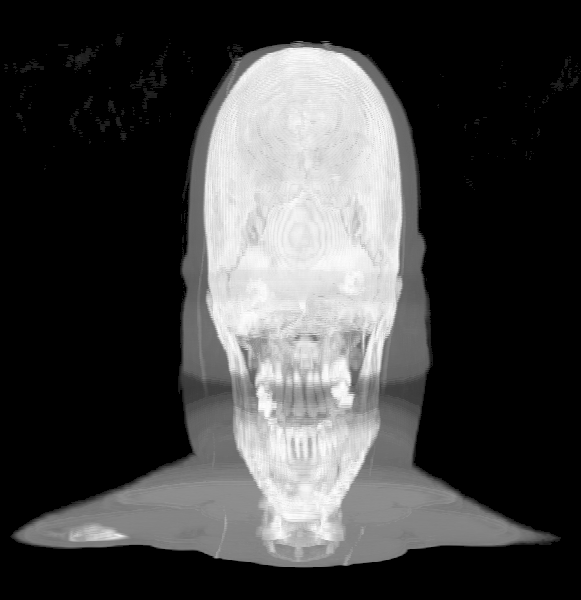
\includegraphics[scale = 0.6]{img/maxi}}
\caption{An example of maximum intensity function output\label{fig:maxi}}
\end{figure}


%https://graphics.ethz.ch/teaching/former/scivis_07/Notes/Handouts/03-raycasting.pdf



\chapter{Conclusion}
\section{Results}
\subsection{Rotation and position}
\subsection{Settings}
\subsubsection{Windowing}
\subsubsection{Thresholding}
\subsubsection{Slice range clipping}
\subsection{Mouse picking}

\section{Disscusion}

\section{Future Development}

\chapter{REFERENCES}

\chapter{Appendix}








\end{document}
